\documentclass[a4paper,11pt]{article}

\usepackage{fullpage}
\usepackage{polski}
\usepackage[T1]{fontenc}
\usepackage[utf8]{inputenc}
\usepackage{times}

\usepackage{amssymb}
\usepackage{amsmath}
\usepackage{textcomp}
\usepackage{graphicx}

\usepackage{hyperref}
\hypersetup{hidelinks}
\urlstyle{same} 



\newcommand{\ang}[1]{(ang. \emph{#1})}


\begin{document}


\title{Kwantowe obliczenia wariacyjne\\ {\normalsize Zastosowania}}

\author{Jarosław Miszczak}
\date{21/12/2022}

\maketitle

\begin{abstract}
Raport przedstawia wybrane zastosowania wariacyjnych algorytmów kwantowych. 
\end{abstract}


%-------------------------------------------------------------------------------
\hypertarget{wprowadzenie}{%
\section{Wprowadzenie}\label{wprowadzenie}}
%-------------------------------------------------------------------------------


\newpage 

%-------------------------------------------------------------------------------
\hypertarget{zastosowania}{%
	\section{Zastosowania}\label{zastosowania}}
%-------------------------------------------------------------------------------


\begin{figure}[ht!]
	\centering
	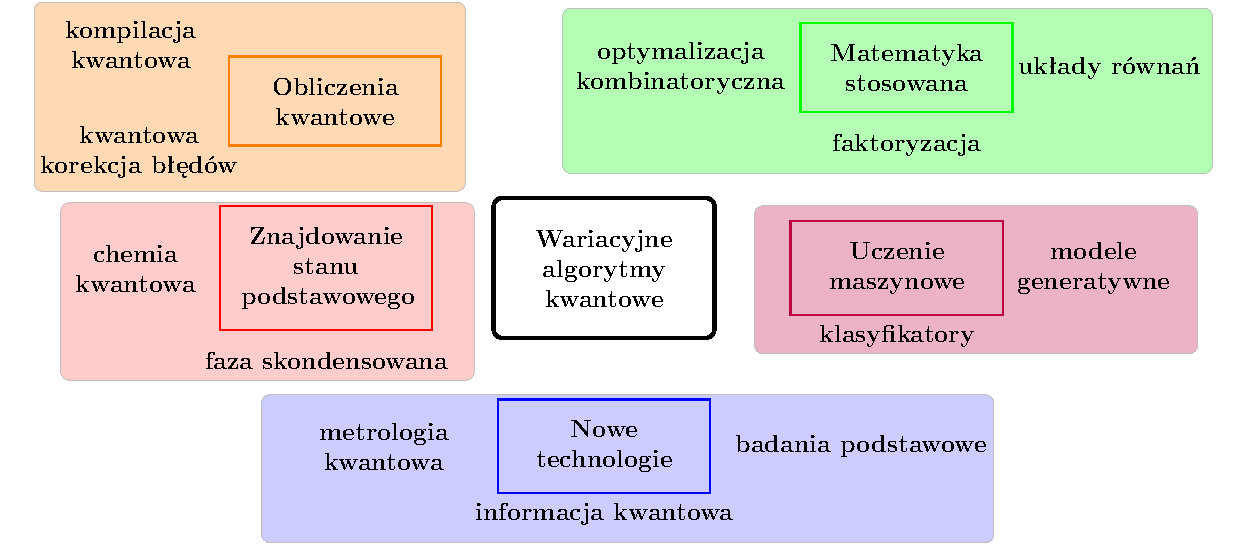
\includegraphics[width=\textwidth]{vqa-applications-pl}
	\caption{Potencjalne dziedziny w których zastosowanie wariacyjnych algorytmów kwantowych może prowadzić do uzyskania przewagi kwantowej.}
\end{figure}

%-------------------------------------------------------------------------------
\hypertarget{matematyczne}{%
	\subsection{Problemy obliczeniowe}\label{matematyczne}}
%-------------------------------------------------------------------------------

%-------------------------------------------------------------------------------
\hypertarget{sec1}{%
	\section{sec1}\label{sec1}}
%-------------------------------------------------------------------------------




\paragraph{}
\paragraph{}
\paragraph{}
\paragraph{}





%-------------------------------------------------------------------------------
\subsection{}
%-------------------------------------------------------------------------------


%-------------------------------------------------------------------------------
\subsection{}
%-------------------------------------------------------------------------------

%-------------------------------------------------------------------------------
\subsection{}
%-------------------------------------------------------------------------------




\newpage 

\hypertarget{literatura}{%
\section*{Literatura}\label{literatura}}

\begin{enumerate}
\def\labelenumi{\arabic{enumi}.}
%\tightlist

\subsection*{Rozwiązywanie układów równań}

\item Huang, H.Y., Bharti, K. and Rebentrost, P., 2021. Near-term quantum algorithms for linear systems of equations with regression loss functions. New Journal of Physics, 23(11), p.113021. \url{https://doi.org/10.1088/1367-2630/ac325f}


\item Bravo-Prieto, C., LaRose, R., Cerezo, M., Subasi, Y., Cincio, L. and Coles, P.J., 2019. Variational quantum linear solver. LA-UR-19-29101, arXiv:1909.05820. \url{https://doi.org/10.48550/arXiv.1909.05820}

\item Pellow-Jarman, A., Sinayskiy, I., Pillay, A. et al. A comparison of various classical optimizers for a variational quantum linear solver. Quantum Inf Process 20, 202 (2021). \url{https://doi.org/10.1007/s11128-021-03140-x}

\subsection*{Obliczenia kwantowe}

\item


\end{enumerate}

\end{document}
